\documentclass[tikz,border=10pt]{standalone}
\begin{document}
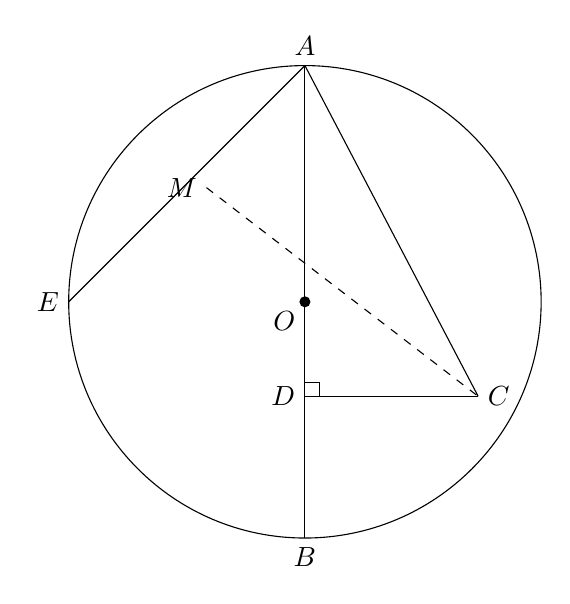
\begin{tikzpicture}[scale=1]

\coordinate (O) at (0,0);
\coordinate (A) at (0,3);
\coordinate (B) at (0,-3);
\coordinate (E) at (-3,0);
\coordinate (C) at (2.2,-1.2);
\coordinate (D) at (0,-1.2);
\coordinate (M) at (-1.25,1.45);

\draw (O) circle (3);

\draw (A) -- (B);
\draw (E) -- (A);
\draw (A) -- (C);
\draw (D) -- (C);
\draw[dashed] (M) -- (C);

\fill (O) circle (2pt);

\draw (0,-1.2) rectangle +(0.18,0.18);

\node[above] at (A) {$A$};
\node[below] at (B) {$B$};
\node[left] at (E) {$E$};
\node[right] at (C) {$C$};
\node[left] at (D) {$D$};
\node[left] at (M) {$M$};
\node[below left] at (O) {$O$};

\end{tikzpicture}
\end{document}
